\subsection*{\large{Выбор архитектуры системы}}
\addcontentsline{toc}{subsection}{Выбор архитектуры системы}

Общий вид системы для автоматического проектирования генеральных планов площадных объектов можно представить в виде
двух независимых друг от друга частей: бизнес и расчётной.
Эти части системы схематично изображены на диаграмме ниже(см. рис\ \ref{pic:architecture__system-diagram}).

\begin{figure}[H]
	\hspace*{-2.5 cm}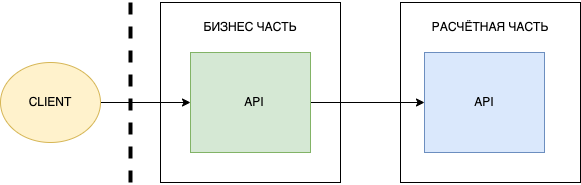
\includegraphics[width=0.6\textwidth, left]{architecture/pictures/system}
	\caption{Общий вид системы}
	\label{pic:architecture__system-diagram}
\end{figure}
\vskip 5 mm

Бизнес часть приложения используется для отображения полученных результатов внешним экспертам со стороны заказчика.
Именно в этой части определены все правила и те объекты, которые используются в экспертной оценке.
В расчётной части системы содержится большое количество объектов внутренней модели данных, используемых для повышения
качества получаемого решения. Эти внутренние объекты никак не могут быть интерпретированы внешними экспертами.

Также стоит отметить, что внутренняя модель данных подвержена сильным изменениям в процессе исследований.
Новые алгоритмы решения задачи могут давать куда более качественный результат, но только с учетом того, что
будут использованы дополнительные структуры данных. В то время как внешняя модель данных относительно стабильна
и представлена объектами целиком и полностью понятными внешним экспертам.

Целью данной работы является проектирование и реализация только расчетной части системы, поэтому на всех остальных
диаграммах представленных в работе рассматривается именно эта часть.
Для решения поставленной задачи предлагается следующая архитектура расчетного модуля.

\begin{figure}[H]
	\hspace*{-2.5 cm}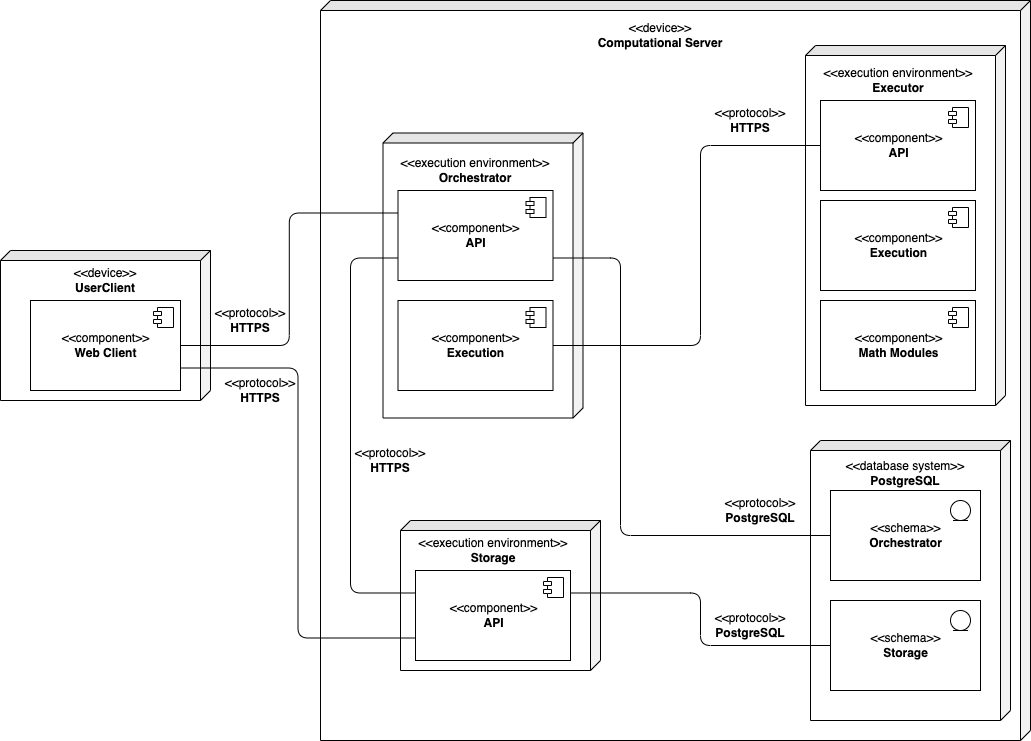
\includegraphics[width=\textwidth, left]{architecture/pictures/deployment_diagram}
	\caption{Диаграмма размещения}
	\label{pic:architecture__deployment-diagram}
\end{figure}
\vskip 5 mm

\noindent Компоненты представленные на диаграмме размещения:
\begin{itemize}
	\item \textbf{Computational Server} -- сервер для запуска расчётных задач.
	\item \textbf{User Client} -- пользовательское устройство для взаимодействия с расчётным сервером.
	\item \textbf{Web Client} -- веб-клиент для получения данных о расчётных задачах.
	\item \textbf{Orchestrator}
	\begin{itemize}
		\item API -- компонент, предоставляющий REST-API для взаимодействия с сервисом.
		\item Execution -- компонент, контролирующий расчет задачи. Последовательно вызывает этапы выполнения задачи.
	\end{itemize}
	\item \textbf{Storage} -- сервис, отвечающий за чтение/хранение данных расчётных задач.
	\begin{itemize}
		\item API -- компонент, предоставляющий REST-API для взаимодействия с сервисом.
	\end{itemize}
	\item \textbf{Executor} -- сервис, отвечающий за запуск математических методов.
	\begin{itemize}
		\item API -- компонент, предоставляющий REST-API для взаимодействия с сервисом.
		\item Execution -- компонент, осуществляющий запуск метода в отдельном процессе, обработку и сохранение решения.
		\item Math Modules -- математическая библиотека \textbf{nd\_plan}, в которой находятся математические методы.
	\end{itemize}
	\item \textbf{PostgreSQL} -- база данных (БД), используемая для хранения данных для расчётных задач.
\end{itemize}

